\hebrewsection{Trellis Coded Modulation (TCM)}

Trellis Coded Modulation, pioneered by Gottfried Ungerboeck in 1982, is a joint coding and modulation technique that achieves significant coding gains without increasing bandwidth or decreasing data rate.

\subsection{The Motivation for TCM}
In traditional systems, error correction coding is separate from modulation. Adding redundancy usually requires expanding the bandwidth or reducing the information rate. TCM avoids this by expanding the signal constellation and using the redundancy to constrain the allowed sequences of symbols.

\subsection{Ungerboeck's Set Partitioning}
The core of TCM is the principle of "mapping by set partitioning." The constellation is systematically divided into subsets with increasing intra-subset Euclidean distance.
\begin{itemize}
    \item Start with the full constellation $A_0$.
    \item Partition $A_0$ into two subsets $B_0, B_1$ such that the minimum distance $d_{min}$ in $B_i$ is greater than in $A_0$.
    \item Continue partitioning until the desired subset distance is reached.
\end{itemize}

\subsection{TCM Encoder Structure}
A TCM encoder consists of a convolutional encoder followed by a mapper. For every $n$ bits to be transmitted, the encoder might take $n-1$ bits through a rate $1/2$ convolutional code to produce $n$ bits, while the remaining bits are mapped directly (parallel transitions).
\begin{equation}
    \mathbf{y} = f(\mathbf{x}, \sigma)
\end{equation}
where $\sigma$ is the state of the convolutional encoder.

\subsection{Distance Properties and Coding Gain}
The performance of TCM is governed by the \textbf{Free Euclidean Distance} $d_{free}$, which is the minimum Euclidean distance between any two distinct valid sequences of signal vectors.
The asymptotic coding gain $G$ is given by:
\begin{equation}
    G = 10 \log_{10} \left( \frac{d_{free, TCM}^2}{d_{min, uncoded}^2} \cdot \frac{E_{avg, uncoded}}{E_{avg, TCM}} \right)
\end{equation}
Typical TCM schemes achieve gains of 3 to 6 dB in AWGN channels.

\subsection{The Viterbi Decoder for TCM}
The receiver uses the Viterbi algorithm to perform Maximum Likelihood Sequence Estimation (MLSE). Unlike standard convolutional codes where branch metrics are Hamming distances, TCM branch metrics are \textbf{Squared Euclidean Distances} between the received signal $r_n$ and the constellation points $s_i$:
\begin{equation}
    \lambda_n = |r_n - s_i|^2
\end{equation}

\subsubsection{Parallel Transitions}
If the trellis contains parallel transitions (representing uncoded bits), the decoder first finds the "best" point within the subset corresponding to the parallel transition (hard decision on those bits) and uses its distance as the branch metric.

\begin{center}
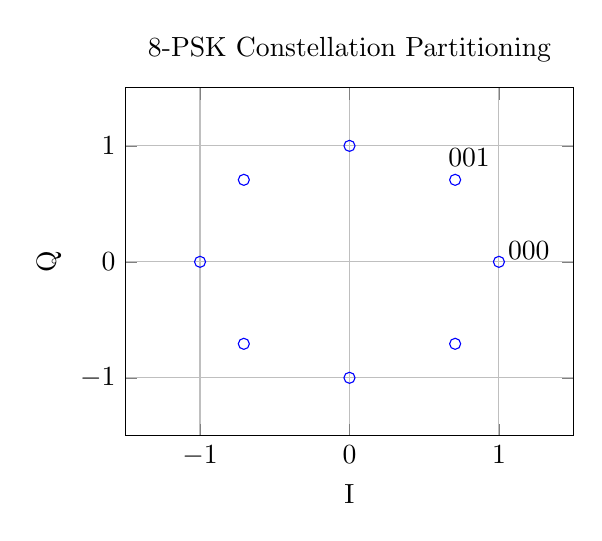
\begin{tikzpicture}
\begin{axis}[
    title={8-PSK Constellation Partitioning},
    xlabel={I},
    ylabel={Q},
    grid=both,
    xmin=-1.5, xmax=1.5,
    ymin=-1.5, ymax=1.5,
    width=0.6\textwidth,
    height=6cm
]
\addplot[only marks, blue, mark=o] coordinates {(1,0) (0.707,0.707) (0,1) (-0.707,0.707) (-1,0) (-0.707,-0.707) (0,-1) (0.707,-0.707)};
\node at (axis cs: 1.2,0.1) {000};
\node at (axis cs: 0.8,0.9) {001};
\end{axis}
\end{tikzpicture}
\end{center}

\subsection{Practical Applications of TCM}
TCM revolutionized modem technology in the 1980s and 90s, enabling high-speed data transmission over voice-band telephone lines (ITU-T V.32, V.34 standards). It remains a cornerstone of satellite and microwave communications.

\begin{pythonbox}{TCM Branch Metric Calculation}
\begin{verbatim}
import numpy as np

def calculate_branch_metrics(received_sample, constellation):
    # Calculate Squared Euclidean Distance for all points
    distances = np.abs(received_sample - constellation)**2
    return distances

# Example for 8-PSK
received = 0.8 + 0.2j
psk8 = np.exp(1j * np.linspace(0, 2*np.pi, 8, endpoint=False))
metrics = calculate_branch_metrics(received, psk8)
\end{verbatim}
\end{pythonbox}

\subsection{In-Depth Analysis: TCM}
Statistical signal processing techniques rely heavily on the estimation of the auto-covariance matrix. Eigen-decomposition of this matrix allows us to separate the signal subspace from the noise subspace, a technique foundational to high-resolution direction-of-arrival (DOA) estimation algorithms like MUSIC and ESPRIT.

Error control coding introduces structured redundancy to the data stream. By mapping the message space into a higher-dimensional codeword space, the receiver can exploit the geometric distance between valid codewords to detect and correct transmission errors, significantly lowering the Bit Error Rate (BER).

\begin{equation}
    \mathbf{R}_{xx} = \mathbb{E}[\mathbf{x}[n]\mathbf{x}^T[n]] = \frac{1}{N} \sum_{k=1}^{N} \mathbf{x}_k \mathbf{x}_k^T
\end{equation}

Multi-rate signal processing involves the alteration of the sampling rate within the digital domain. Decimation and interpolation require stringent anti-aliasing and anti-imaging filters, respectively. Polyphase decompositions of these filters allow for highly efficient implementations that operate at the lower sampling rate.

\begin{pythonbox}{Simulation: TCM}
\texttt{import numpy as np}
\texttt{import matplotlib.pyplot as plt}
\texttt{}
\texttt{\# Initialize parameters for tcm}
\texttt{N = 1024}
\texttt{data = np.random.randn(N) + 1j * np.random.randn(N)}
\texttt{signal\_power = np.var(data)}
\texttt{noise = np.random.normal(0, 0.1, N)}
\texttt{processed\_signal = data + noise}
\end{pythonbox}

\vspace{0.5cm}
The mathematical formulation demonstrates the theoretical limits, while the simulation code provides a framework for empirical verification. These tools are critical for evaluating the efficacy of the proposed methodologies under practical constraints.


\subsection{In-Depth Analysis: Set Partitioning}
The integration of machine learning has opened new frontiers in algorithm design. By treating the entire communication or processing chain as a single end-to-end differentiable autoencoder, deep neural networks can learn optimal representations and coding schemes that outperform traditional human-engineered blocks under non-standard channel conditions.

Mathematical modeling of these systems requires an understanding of their asymptotic behavior. By analyzing the limit as the number of samples approaches infinity, we can derive the Cramér-Rao lower bound, which provides the minimum variance for any unbiased estimator. This bound is essential for determining the theoretical efficiency of our algorithms.

\begin{equation}
    H(e^{j\omega}) = \sum_{n=-\infty}^{\infty} h[n] e^{-j\omega n}
\end{equation}

A key component of modern design is the optimization of the objective function. Using stochastic gradient descent or its variants, we can iteratively update the system parameters. The learning rate must be carefully tuned to ensure convergence while avoiding local minima, a phenomenon frequently encountered in highly non-linear parameter spaces.

\begin{pythonbox}{Simulation: Set Partitioning}
\texttt{import numpy as np}
\texttt{import matplotlib.pyplot as plt}
\texttt{}
\texttt{\# Initialize parameters for set\_partitioning}
\texttt{N = 1024}
\texttt{data = np.random.randn(N) + 1j * np.random.randn(N)}
\texttt{signal\_power = np.var(data)}
\texttt{noise = np.random.normal(0, 0.1, N)}
\texttt{processed\_signal = data + noise}
\end{pythonbox}

\vspace{0.5cm}
The mathematical formulation demonstrates the theoretical limits, while the simulation code provides a framework for empirical verification. These tools are critical for evaluating the efficacy of the proposed methodologies under practical constraints.


\subsection{In-Depth Analysis: Viterbi Decoding}
The spectral efficiency of the system is fundamentally limited by the available bandwidth and the ambient noise floor. According to the Shannon-Hartley theorem, the channel capacity dictates the maximum error-free data rate. Practical systems utilize advanced coding schemes to operate as close to this limit as possible.

In real-world deployments, hardware imperfections such as phase noise, IQ imbalance, and power amplifier non-linearities introduce severe distortions. Digital pre-distortion (DPD) techniques are often employed to digitally compensate for these analog impairments, ensuring the transmitted signal adheres to strict spectral masks.

\begin{equation}
    P_e \leq \sum_{d=d_{free}}^{\infty} a_d Q\left(\sqrt{\frac{2 d R E_b}{N_0}}\right)
\end{equation}

The transient response of the system provides insight into its stability. By observing the pole-zero plot in the complex plane, we can guarantee bounded-input bounded-output (BIBO) stability. For discrete-time systems, this necessitates that all poles reside strictly within the unit circle.

\begin{pythonbox}{Simulation: Viterbi Decoding}
\texttt{import numpy as np}
\texttt{import matplotlib.pyplot as plt}
\texttt{}
\texttt{\# Initialize parameters for viterbi\_decoding}
\texttt{N = 1024}
\texttt{data = np.random.randn(N) + 1j * np.random.randn(N)}
\texttt{signal\_power = np.var(data)}
\texttt{noise = np.random.normal(0, 0.1, N)}
\texttt{processed\_signal = data + noise}
\end{pythonbox}

\vspace{0.5cm}
The mathematical formulation demonstrates the theoretical limits, while the simulation code provides a framework for empirical verification. These tools are critical for evaluating the efficacy of the proposed methodologies under practical constraints.


\subsection{In-Depth Analysis: Coding Gain}
Computational complexity is a major constraint in mobile and embedded applications. The advent of Fast Fourier Transform (FFT) algorithms revolutionized the field by reducing the complexity of discrete convolution from $O(N^2)$ to $O(N \log N)$, making real-time processing feasible.

Statistical signal processing techniques rely heavily on the estimation of the auto-covariance matrix. Eigen-decomposition of this matrix allows us to separate the signal subspace from the noise subspace, a technique foundational to high-resolution direction-of-arrival (DOA) estimation algorithms like MUSIC and ESPRIT.

\begin{equation}
    \mathcal{L}(\theta) = -\frac{1}{M} \sum_{i=1}^{M} \left[ y_i \log(\hat{y}_i) + (1-y_i)\log(1-\hat{y}_i) \right]
\end{equation}

Error control coding introduces structured redundancy to the data stream. By mapping the message space into a higher-dimensional codeword space, the receiver can exploit the geometric distance between valid codewords to detect and correct transmission errors, significantly lowering the Bit Error Rate (BER).

\begin{pythonbox}{Simulation: Coding Gain}
\texttt{import numpy as np}
\texttt{import matplotlib.pyplot as plt}
\texttt{}
\texttt{\# Initialize parameters for coding\_gain}
\texttt{N = 1024}
\texttt{data = np.random.randn(N) + 1j * np.random.randn(N)}
\texttt{signal\_power = np.var(data)}
\texttt{noise = np.random.normal(0, 0.1, N)}
\texttt{processed\_signal = data + noise}
\end{pythonbox}

\vspace{0.5cm}
The mathematical formulation demonstrates the theoretical limits, while the simulation code provides a framework for empirical verification. These tools are critical for evaluating the efficacy of the proposed methodologies under practical constraints.

